\section{Charged particles and magnetic fields}\index{EP}

When a collision occurs, a very large number of particles are produced.  Figure ~\ref{fig:trk1} shows a schematic view.

\begin{figure}[h]
\centering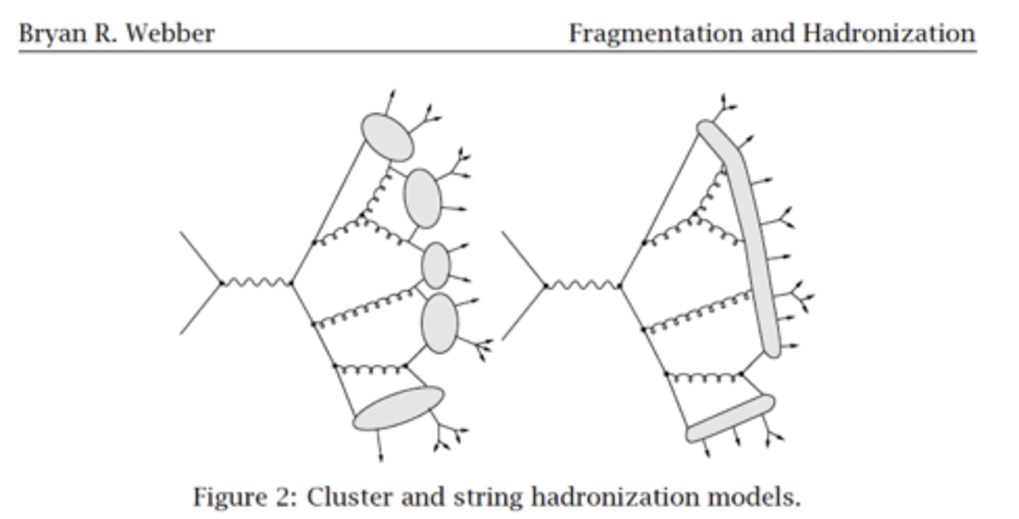
\includegraphics[scale=0.5]{./Trackers/Pictures/fig1.pdf}
\caption{Cartoon of particle production in hadronic collisions}
\label{fig:trk1}
\end{figure}

Some of the particles have an electric charge (electrons, charged pions,etc). Some are electrically neutral (photons, neutrons, neutral pions).  The first kind of detector we will discuss can be used to measure the momenta of charged particles.
Almost all modern particle physics detectors (an exception being the first version of the Dzero detector) feature large solenoidal magnets.  A solenoid is a current-carrying wire wrapped into a cylindrical form. Inside the cylinder, there is an (approximate) uniform magnetic field, with the magnetic field lines parallel to the cylinder's (z) axis. 
\begin{figure}[h]
\centering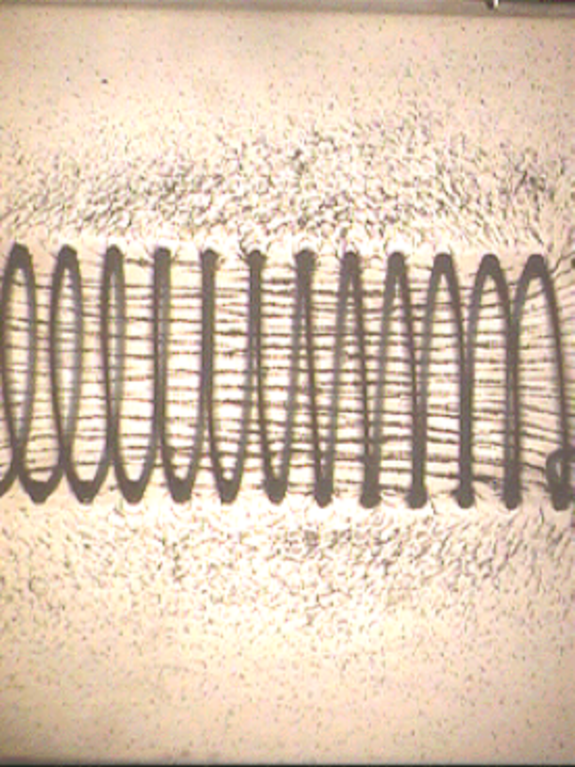
\includegraphics[scale=0.5]{./Trackers/Pictures/fig2.pdf}
\caption{Iron filings are used to show the magnetic field lines inside a solenoidal magnet.}
\label{fig:trk2}
\end{figure}

As you may remember from your high school physics class, a charged particle moving in a magnetic field will experience a force given by:
\begin{center}$\vec{F}$ = q$\vec{v}$$\times$$\vec{B}$ \end{center}
 where $\vec{v}$ is the velocity of the particle and q is its electric charge. The direction of the force is perpendicular to both the velocity and the field. The magnitude is qv$_{T}$B, where v$_{T}$ is the magnitude of the component of the velocity perpendicular to the magnetic field. You may remember that when the force is perpendicular to the velocity, the resulting motion is circular.  For circular motion, you may remember that the acceleration is given by v$^{2}$/r. So we have:
\begin {equation*} \hspace {58 mm}
m\dfrac{v_{T}^{2}}{r} = qv_{T}B
\end{equation*}
or (so that it will work with relativity, we change the mv$_{T}$ to p$_{T}$). This equation is in cgs units. In convenient units (r in m, p$_{T}$ in GeV, B in Tesla, q in units of e), the equation is:
\begin{center} p$_{T}$ = .3qrB \end{center}
Now, imagine a particle produced at the center of the solenoid pictured above with momentum p=(p$_{x}$,p$_{y}$,p$_{z}$). Since the magnetic field is along the z direction, the force will be in the x-y plane. The resulting motion will be a spiral around the z axis. In that plane the motion will be circular.  The component of velocity in the z direction will be unaffected, so in the x-z or y-z planes, the motion will be a straight line.

As you call tell from the equation above, if we can measure the radius of curvature of this motion in the x-y plane, we get the component of momentum transverse to the z (beam) axis.  If we can also measure the polar and azimuthal angles, we can get the 4-momenta of the particle from the transverse momentum using elementary trigonometry.

As you can see, the higher momentum the track, the straighter its trajectory will be.  Low momentum tracks will bend more.  Very low momentum tracks may even be able to make a complete circle or more before leaving the detector. 

\section{Detecting the trajectory of the charged particle}
In order to measure the radius of curvature, we need to know the path the particle takes as it emerges from the collision, and we have to measure this path without altering or disturbing the momenta of the particle.  We need some material that produces a signal we can detect and it should be thin and low Z so that the particle does not lose much energy or scatter much while going through it. 
 
There are two common detection medium used: gas and silicon.  Gas has the advantage of being cheap and very thin.  However, it typically can be used to measure a position on the trajectory with an accuracy of a few hundred microns, and it cannot handle a very high radiation environment.  Silicon is thicker and more expensive, but can give measurements to a few 10's of microns and can handle a higher radiation environment.  Both are used to produce a current that can be detected.  For gas-based detectors, the particles ionize the gas, and the freed electrons are collected on wires that are at HV.  As the freed electrons approach the wires, an ``avalanche''  process results, because the electrons accelerate in the electric field around the wire.  When they reach a high enough energy, they ionize more gas, and these extra electrons are accelerated until a measurable current is created. In silicon, ionization is again the process that produces the signal, but high voltage is not required to collect the charge due to the short distances involved.
\noindent
The CMS tracker is silicon based.  A schematic is shown in figure ~\ref{fig:trk3}.

\begin{figure}[h]
\centering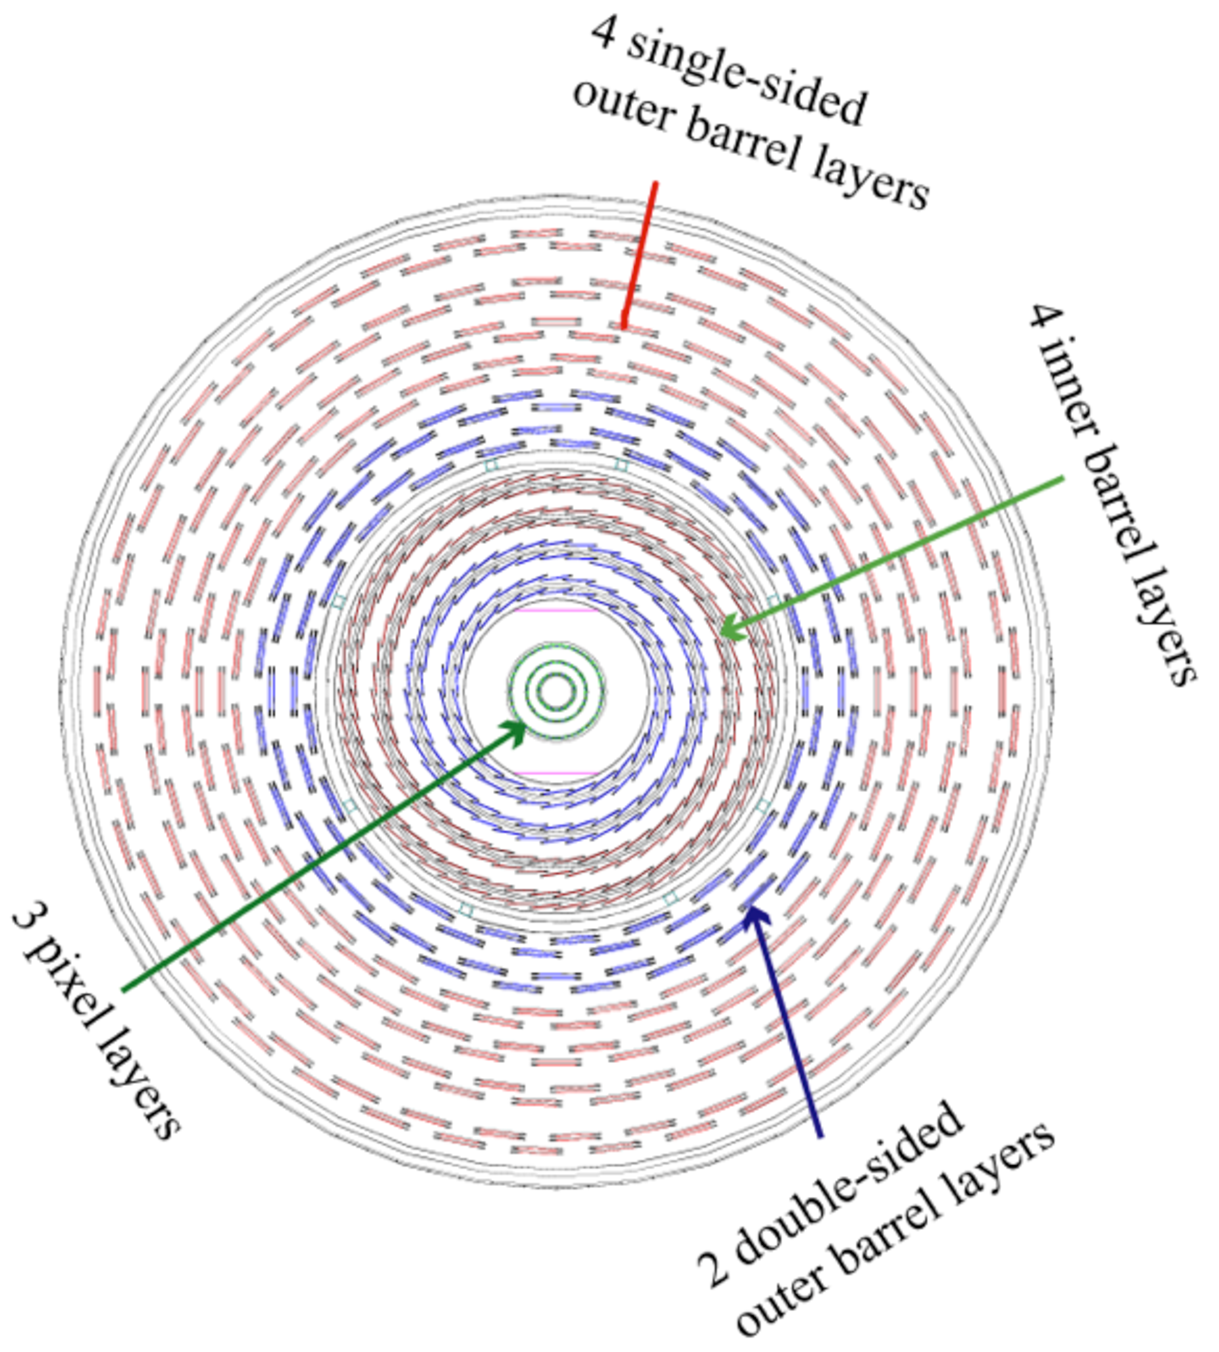
\includegraphics[scale=0.5]{./Trackers/Pictures/fig3.pdf}
\caption{ A schematic of the CMS silicon tracker.}
\label{fig:trk3}
\end{figure}
\noindent
As you can see, the tracker measures the track position at 15 positions along its trajectory. The ``strips'' that you see in each layer are segmented into individual detectors, with each strip of the silicon detectors reaching out to a radius of 130 centimeters. 
\section{Tracker Resolutions}
Reconstruction of tracks from the detector information takes place in two steps. First, a ``pattern recognition'' algorithm decides which ``hits''(localized detector information) go together into a single track. This is a complicated process, and very detector and collider specific. The next step,``fitting'', uses this information to reconstruct the transverse momentum, angles (and distance of closest approach to the beam axis, for tracks produced from decays of long-lived particles).  
Let's consider the fitting part.  Here, we will only consider the resolution on p$_{T}$, which is a 2 dimensional calculation, using the information in the plane transverse to the beam direction.   

For a track produced at the vertex, and ignoring non-uniformities in the magnetic field and scattering by the particle in the material of the detector, the track's trajectory will trace out a circle that includes the origin.  The general equation for a circle that satisfies these constraints is:
\begin{equation*}\hspace{50 mm}
(x-a)^{2}+(y-b)^{2}=a^{2}+b^{2}
\end{equation*}
where a and b are the coordinates of the center of the circle and $\sqrt{a^{2}+b^{2}}$ is the radius of the circle, which is what we really want to find to get our transverse momentum.
When fitting, it is often useful to do a transformation of variables to linearize the equation.  Consider the transformation:
\begin{equation*}\hspace {54mm}
u=\frac{x}{x^{2}+y^{2}} \hspace{5 mm} v=\frac{y}{x^{2}+y^{2}}
\end{equation*}
\noindent
In these variables, the equation of a circle is:
\begin{equation*}\hspace{58 mm}
v =-\frac{a}{b}u+\frac{1}{2b}
\end{equation*}
If you compare this to the equation of straight line, you will see that the slope of v versus u gives you -$\frac{a}{b}$ and the intercept gives $\frac{1}{2b}$.

\section{Fitting a straight line}
Fitting is usually done by minimizing a $\chi^{2}$. Remember that this is defined as: 
\begin{equation*}\hspace{48 mm}
\chi^2=\sum \frac{(data-theory)^{2}}{error^{2}}
\end{equation*}
For a fit to a straight line, it is easy to calculate what values for the slope and intercept will minimize this quantity. For a straight line, y=mx+b. Let z=y-mx+b. For a perfect fit, z will be 0. The $\chi^{2}$ would then become: 
\begin{equation*}\hspace{60 mm}
\chi^2=\sum \frac{(z)^{2}}{\sigma_{z}^{2}}
\end{equation*}
where $\sigma_{z}^{2}$ is the uncertainty(error)in z. What values of m and b will minimize this $\chi^{2}$? 

\begin{align*} \hspace{44 mm}
\sigma_{z}&=\sqrt{(\frac{\partial z }{\partial y} \sigma_{}y)^{2}+(\frac{\partial z}{\partial x}\sigma_{x})^{2}}\\
\hspace{9mm}&=\sqrt{(\sigma_{y})^{2}+(m\sigma_{x})^{2}}
\end{align*}
\begin{equation*}\hspace{35mm}
\chi^{2}=\sum_{data}\frac{(z-0)^{2}}{\sigma_{z}^{2}}=\sum_{data}\frac{(y-mx-b)^{2}}{(\sigma_{y}^{2})+(m\sigma_{x}^{2})}
\end{equation*}
\noindent
If we consider the simpler case, where the errors on x are negligible, we can simplify the derivation to: 
\begin{equation*}\hspace{48mm}
\chi^{2}=\sum_{data}\frac{(y-mx-b)^{2}}{(\sigma_{y}^{2})}
\end{equation*}
To minimize this, we use our knowledge of elementary calculus, which tells us that a function has a minimum or maximum when its derivative is zero.
\begin{align*}\hspace{40mm}
\frac{\partial\chi^2  }{\partial b}=-2\sum_{i}\frac{1}{\sigma_{i}^{2}}(y_{i}-b-mx_{i})=0\\
\frac{\partial\chi^2  }{\partial m}=-2\sum_{i}\frac{x_{i}}{\sigma_{i}^{2}}(y_{i}-b-mx_{i})=0
\end{align*}
Rearranging: 
\begin{align*}\hspace{35mm}
\left(\sum_{i}\frac{y_{i}}{\sigma{i}^{2}}\right)=b\left(\sum_{i}\frac{{1}}{\sigma{i}^{2}}\right)+m\left(\sum_{i}\frac{x_{i}}{\sigma{i}^{2}}\right)\\
\left(\sum_{i}\frac{x_{i}y_{i}}{\sigma{i}^{2}}\right)=b\left(\sum_{i}\frac{{x_{i}}}{\sigma{i}^{2}}\right)+m\left(\sum_{i}\frac{x_{i}^{2}}{\sigma{i}^{2}}\right)
\end{align*}
Solving: 
\begin{align*}\hspace{23mm}
b=\frac{1}{\Delta}\left[ \left(\sum_{i}\frac{x_{i}^{2}}{\sigma_{i}^{2}} \right ) \left(\sum_{i}\frac{y_{i}}{\sigma_{i}^{2}} \right)-\left( \sum_{i}\frac{x_{i}}{\sigma_{i}^{2}}\right)\left(\sum_{i}\frac{x_{i}y_{i}}{\sigma_{i}^{2}}\right )\right]\\
m=\frac{1}{\Delta}\left[ \left(\sum_{i}\frac{1}{\sigma_{i}^{2}} \right ) \left(\sum_{i}\frac{x_{i}y_{i}}{\sigma_{i}^{2}} \right)-\left( \sum_{i}\frac{x_{i}}{\sigma_{i}^{2}}\right)\left(\sum_{i}\frac{y_{i}}{\sigma_{i}^{2}}\right )\right]
\end{align*}
\noindent
Where: 
\begin{equation*}\hspace{41mm}
\Delta=det\begin{bmatrix}
\left(\sum_{i}\frac{1}{\sigma_{i}^{2}} \right )&\left(\sum_{i}\frac{x_{i}}{\sigma_{i}^{2}} \right)\\ \\
\left(\sum_{i}\frac{x_{i}}{\sigma_{i}^{2}} \right)&\left(\sum_{i}\frac{x_{i}^{2}}{\sigma_{i}^{2}}\right)
\end{bmatrix}
\end{equation*}

\section{Project}
Write a little Monte Carlo program that will generate tracks with a transverse momentum of 1 GeV produced at the origin, in a uniform magnetic field along the z axis of 3 Tesla and transversing a detector that takes measurements at 12 different layers, uniformly spaced in r (the radial distance from the beam axis) between 0 and 1.5 m. Imagine each layer measures the r coordinate perfectly and the coordinate perpendicular to that with an accuracy of 10$\mu$m. Use MC to generate the ``true'' hits, transform them from r-$\varphi$ to x-y, smear them to get the measured hit positions, and then fit the ``smeared''hits to measured radius of curvature. What resolution would you predict?  What resolution do you get?  How does it change if you produce 10 GeV tracks instead? 100 GeV tracks?
\section{Further Reading}
$\cdot$ \url{http://pdg.lbl.gov/2011/reviews/rpp2011-rev-particle-detectors-accel.pdf} Section 28.6, 28.7\\
\noindent
$\cdot$\url{http://www.sciencedirect.com/science/article/pii/S0168900211020389}



















